%% main.tex — WikiKGQA Challenge @ ISWC 2026 (English version)
%% Compilation : pdfLaTeX
%%
%% Fonts : Libertinus Serif (roman), Libertinus Sans (headings), Libertinus
%% Mono (\texttt), Libertinus Math (math). The ceurart class already loads
%% `libertinus` (Serif/Sans/Mono); we add `libertinust1math` to match maths.
\documentclass[]{ceurart}

\sloppy

%% --- Libertinus fonts -----------------------------------------------------
%% ceurart.cls already loads \RequirePackage[T1]{fontenc} and \RequirePackage{libertinus}.
%% We only add the matching math font.
\usepackage{libertinust1math}   %% Libertinus Math (type 1, pdfLaTeX compatible)

%% --- Tables and figures ---------------------------------------------------
\usepackage{booktabs}
\usepackage{tabularx}
\usepackage{array}
\usepackage{url}
\usepackage{xcolor}
\usepackage{graphicx}
\graphicspath{{images/}}
\usepackage{siunitx}

\begin{document}

\copyrightyear{2026}
\copyrightclause{Copyright for this paper by its authors.
  Use permitted under Creative Commons License Attribution 4.0 International (CC BY 4.0).}

\conference{WikiKGQA Challenge @ ISWC 2026: International Semantic Web Conference, October 2026, Nara, Japan}

\title{TF-IDF Example Retrieval and Execution-Guided Selection for Few-Shot Text-to-SPARQL over Wikidata with Open-Weight LLMs}

\tnotemark[1]
\tnotetext[1]{System paper for the WikiKGQA~@~ISWC~2026 challenge, \texttt{en-with-mentions} and \texttt{es-with-mentions} tracks.}

\author[1]{Kenmegne Fokam Emeric Cyrille}[%
orcid=0009-0001-4232-2361,
email=emeric.kenmegne@facsciences-uy1.cm,
]
\cormark[1]

\author[1]{Tela Tela Gilbert Ebenezer}[%
email=gilbert.tela@facsciences-uy1.cm,
]

\address[1]{Department of Computer Science, University of Yaound\'e~I, Yaound\'e, Cameroon}

\cortext[1]{Corresponding author.}

\begin{abstract}
We report on our participation in the two \emph{with-mentions} tracks (English and Spanish) of the WikiKGQA~@~ISWC~2026 challenge, whose task is to translate a natural-language question into a SPARQL query executable against a Wikidata subgraph. Our system chains four stages: a TF-IDF retriever that selects three similar training examples, a few-shot prompt sent to an open-weight LLM, generation of five candidates with mixed temperatures (one deterministic, four at 0.7), and selection of the first candidate returning a non-empty result on the challenge endpoint. On the development split (100 questions per language) we obtain macro F1 = 0.634 in English and 0.607 in Spanish; on the official Codabench test (75 questions per language) scores reach 0.650 and 0.630. An error analysis isolates two resistant categories: type-filter questions in \emph{``which/qu\'e''}, which rely on the \texttt{P31/P279*} chain that is incomplete on the endpoint, and \texttt{COUNT} queries, for which the LLM frequently forgets the aggregate. The pipeline uses only open-weight models (\texttt{gpt-oss-120b}, \texttt{llama-3.3-70b}) served free of charge through Groq Cloud.
\end{abstract}

\begin{keywords}
  Knowledge Graph Question Answering \sep
  Wikidata \sep
  Large Language Models
\end{keywords}

\maketitle

%==============================================================================
\section{Introduction}
\label{sec:intro}
%==============================================================================
Knowledge Graph Question Answering (KGQA) aims at querying an RDF graph in natural language. On a collaborative graph such as Wikidata~\cite{vrandecic2014wikidata}, the difficulty is twofold: mentions must first be disambiguated to the right Q-identifiers, and the logical structure of the question then translated into a coherent graph pattern. This second step involves picking the right properties and handling aggregates, filters and joins, all in a multilingual setting. The WikiKGQA~@~ISWC~2026 challenge provides \num{497}~bilingual (English/Spanish) question–SPARQL pairs built on top of QAWiki, a dedicated QLever~\cite{bast2017qlever} endpoint serving a simplified view of Wikidata frozen for the duration of the challenge, and an online Codabench evaluation using QALD macro F1~\cite{perevalov2022qald10}. We participate in the two \emph{with-mentions} tracks, where the Q-identifiers of the mentioned entities are provided with the question, isolating the query-generation problem. Our contributions are: (i)~a four-stage pipeline — TF-IDF retrieval, few-shot prompting, multi-candidate generation, execution-guided selection — built entirely on open-weight LLMs; (ii)~a dev and test evaluation of both tracks, with macro F1 of 0.634/0.607 on dev and 0.650/0.630 on test; (iii)~a structured error analysis that isolates the two most resistant question categories, namely type-filter questions and \texttt{COUNT} queries.

%==============================================================================
\section{Related Work}
\label{sec:related}
%==============================================================================
The QALD series~\cite{usbeck2017qald} has set the evaluation protocol still used today (macro F1 on the union of answers), and QALD-10~\cite{perevalov2022qald10} marked its migration to Wikidata. Classical approaches based on supervised semantic parsers or hand-written templates score well on distributions seen at training time but generalise poorly to new reformulations; end-to-end \emph{text-to-SPARQL} generation with a fine-tuned seq2seq model produces syntactically valid queries but suffers from hallucinated IRIs — the model generates plausible-looking properties that do not exist in the target graph. Since GPT-3~\cite{brown2020gpt3}, several works have shown that an instruction-tuned LLM produces competitive SPARQL queries from a handful of in-context examples~\cite{li2023fewshot}, and KAPING~\cite{baek2023kaping} further injects the graph neighbourhood in the prompt. We inherit from this line the retrieval-guided few-shot principle but deliberately choose an unlearned retriever (TF-IDF~\cite{salton1988term}) so that the pipeline remains reproducible from public resources. In parallel, Wang \emph{et al.}~\cite{wang2022selfconsistency} popularised the idea that sampling multiple outputs and voting improves LLM robustness; Self-Refine~\cite{madaan2023selfrefine} extends this family by asking the model to critique and rewrite its own output. Our execution-guided selection follows the same spirit but avoids the critique step: the SPARQL endpoint itself acts as an oracle, separating empty queries from exploitable ones.

%==============================================================================
\section{Task and Data}
\label{sec:task}
%==============================================================================
For each natural-language question, the challenge asks for both an executable SPARQL query and the corresponding answer set: list of Q-identifiers for \texttt{SELECT} queries, a boolean for \texttt{ASK}, an integer for \texttt{COUNT}. Four tracks are offered by the organisers: two with entity mentions given (EN and ES) and two without. Our submission covers the two \emph{with-mentions} tracks. The QAWiki corpus is distributed as JSON derived from the QALD schema. Each item bundles an identifier, the question in both languages, the list of entity mentions (surface form followed by Q-identifier), the reference SPARQL query, and the list of expected answers (Fig.~\ref{fig:dataset}). Version 2026.2 used in this paper contains \num{497}~questions, split officially into \num{317}~train, \num{100}~dev and \num{80}~test (of which 75 are actually scored). The target graph is served by a challenge-specific QLever~\cite{bast2017qlever} endpoint. This detail matters: unlike the public Wikidata endpoint, the served view is \emph{simplified} and some hierarchies — notably the transitive closure \texttt{P31/P279*} — are incomplete, so a syntactically perfect query may return an empty result simply because the queried property is not materialised. We exploit this in the execution-guided selection (Sect.~\ref{sec:method}). The official metric is QALD macro F1~\cite{perevalov2022qald10}: for each question, F1 is the harmonic mean of precision and recall computed over the returned Q-identifiers, and the overall score is the mean of per-question F1s. We also report, for analysis purposes, the number of perfectly answered and completely missed questions.

\begin{figure}[h]
\centering
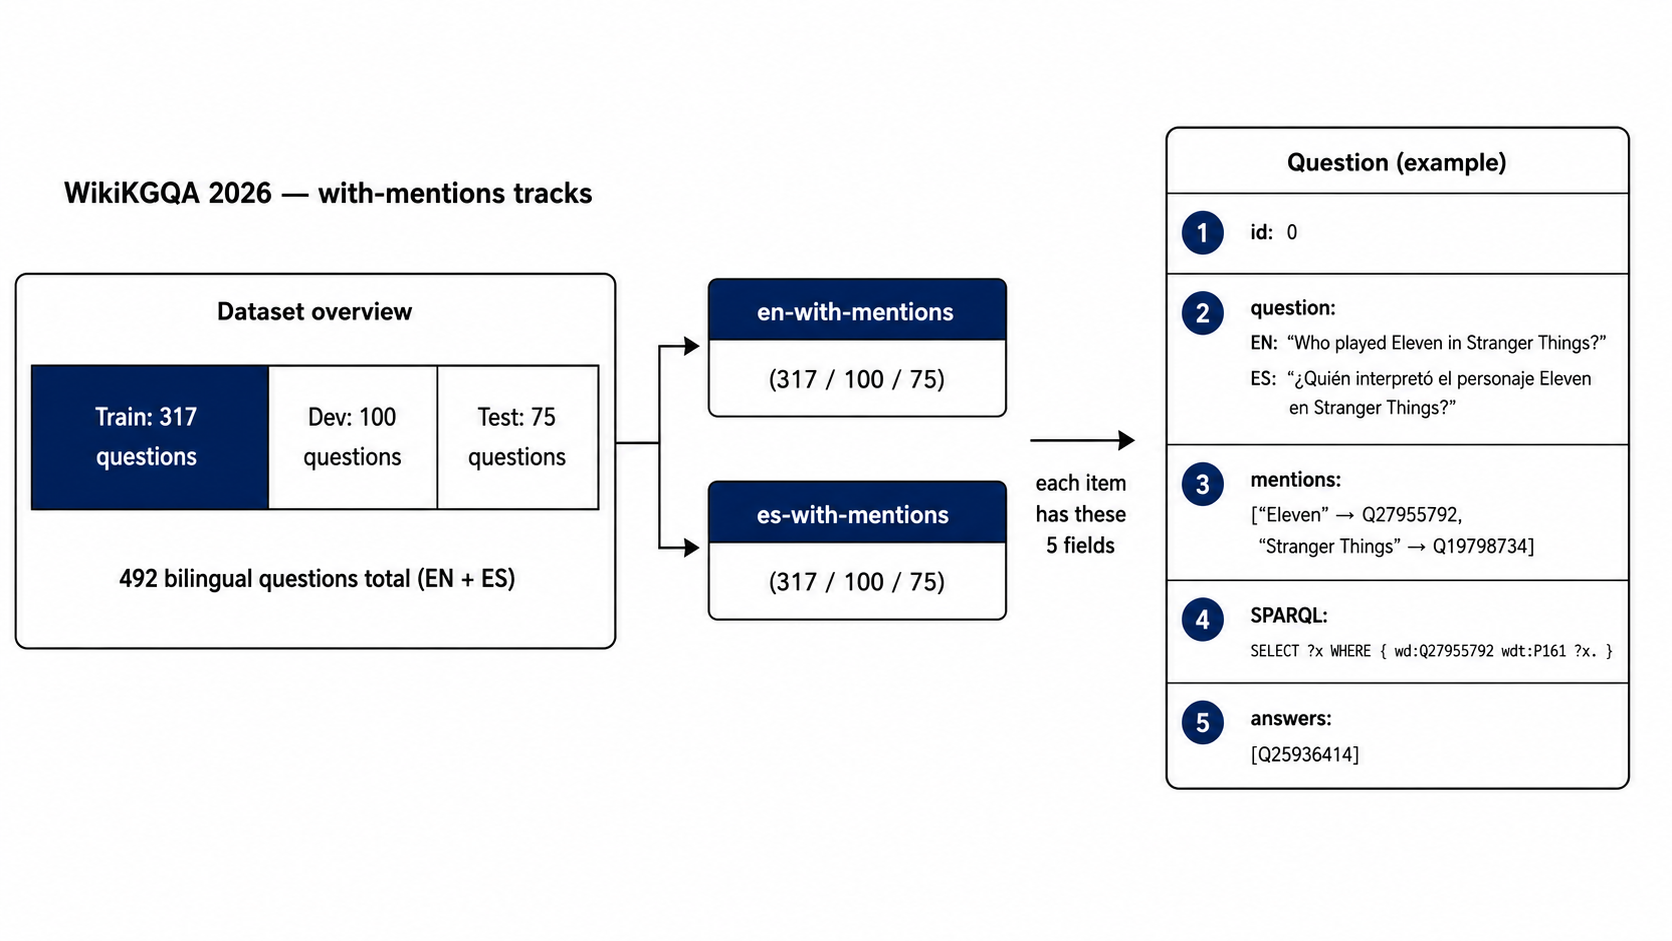
\includegraphics[width=0.9\linewidth]{data.png}
\caption{Format of a QAWiki item: bilingual question, entity mentions with Q-identifiers, reference SPARQL query, expected answers.}
\label{fig:dataset}
\end{figure}

%==============================================================================
\section{Proposed System}
\label{sec:method}
%==============================================================================
Our pipeline, referred to as P3 below, is linear and uses neither an agent nor a learned re-ranker. It takes a question and its mentions as input and produces a SPARQL query together with its answer set (Fig.~\ref{fig:pipeline}). For each target question, the retriever selects the three nearest neighbours in the training corpus in terms of cosine similarity between TF-IDF~\cite{salton1988term} vectors built on word $n$-grams with $n\in\{1,2\}$; a light heuristic infers the target query type (\texttt{ASK}, \texttt{COUNT}, \texttt{SELECT}) from question keywords and, at comparable similarity, favours neighbours of the same type. The vectoriser trains in under a second on the \num{317}~training questions. The prompt consists of three blocks (Fig.~\ref{fig:processing}): a system instruction fixing the expected format and forbidding \texttt{PREFIX} declarations (they will be prepended automatically at execution time); the three examples formatted as \texttt{(question, mentions, SPARQL)} triples, each wrapped in a \texttt{```sparql~\dots~```} fenced block; the target question with its mentions in the same format. For each question we call the LLM five times: one call at zero temperature (best-guess deterministic candidate) and four calls at temperature 0.7 (diversification). Each candidate is extracted from its code block, prefixed with the standard Wikidata \texttt{PREFIX} declarations, and sent to the endpoint via HTTP with a 30~s timeout; 429 and 5xx codes are handled by an adaptive retry layer that respects Groq's \texttt{Retry-After}. The selection rule is straightforward: we scan candidates in order (deterministic first, then stochastic) and return the answers of the first candidate producing at least one row. If all candidates return an empty set, we keep the deterministic output; this covers the rare cases where the gold answer is actually empty (negative \texttt{ASK}, \texttt{SELECT} with \texttt{MINUS}). The pipeline does not differentiate between languages at the code level: retriever, prompt format and selection logic are identical; TF-IDF nonetheless builds two separate vocabularies, one per language.

\begin{figure}[h]
\centering
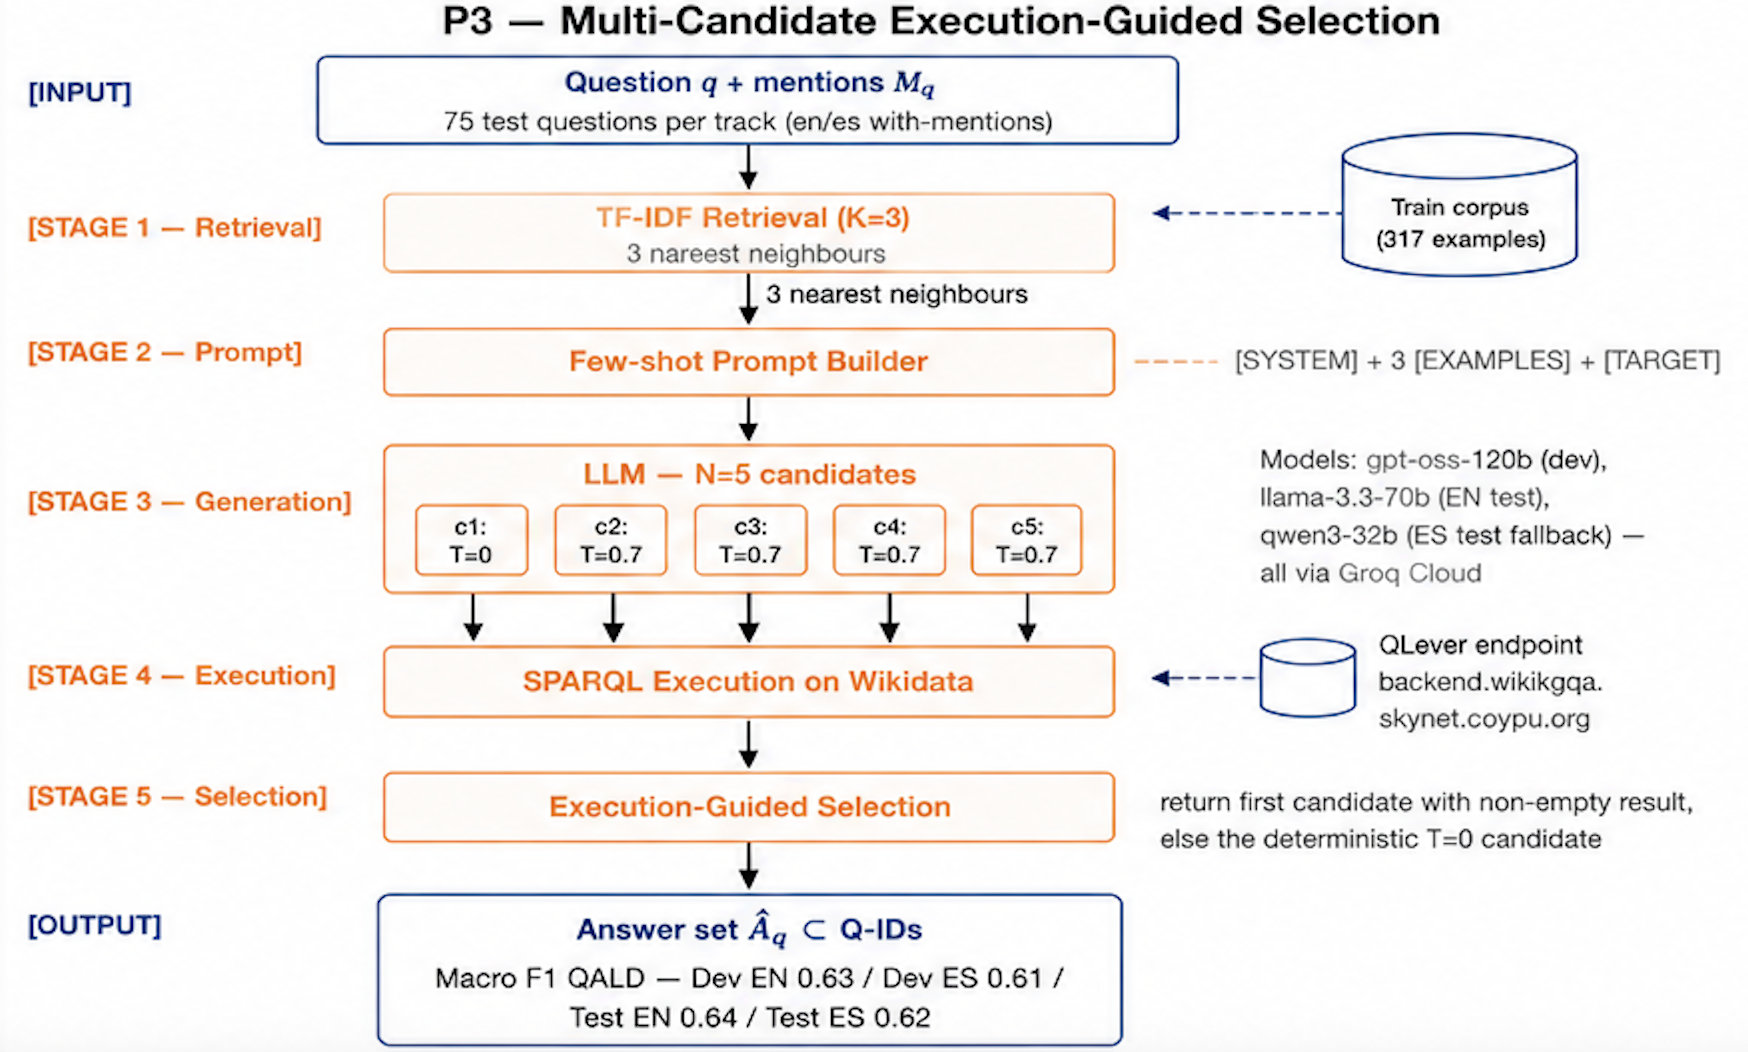
\includegraphics[width=0.78\linewidth]{solution.png}
\caption{The P3 pipeline. (1)~TF-IDF retrieval of the three nearest neighbours; (2)~few-shot prompt construction; (3)~LLM generation of five SPARQL candidates (one at $T{=}0$, four at $T{=}0.7$); (4)~execution of every candidate on the challenge endpoint; (5)~selection of the first non-empty candidate.}
\label{fig:pipeline}
\end{figure}

\begin{figure}[h]
\centering
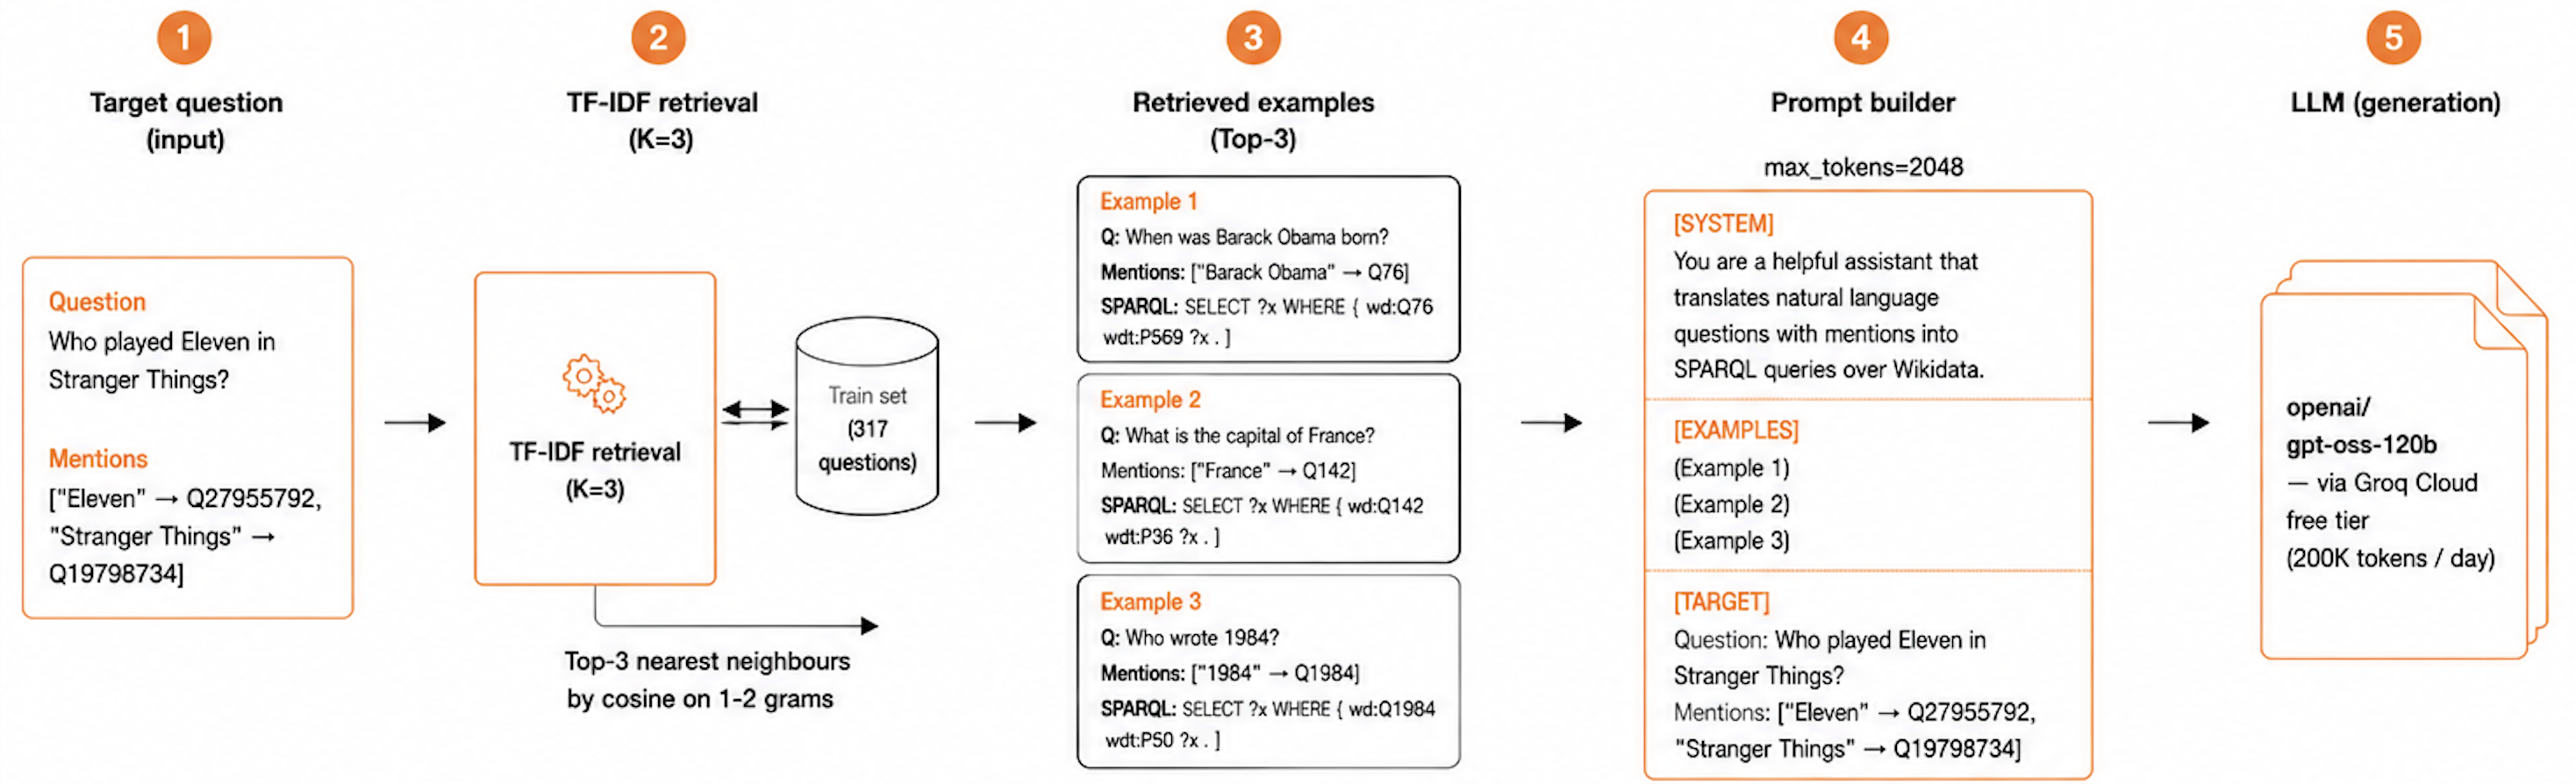
\includegraphics[width=0.95\linewidth]{processing.png}
\caption{Few-shot prompt construction. The target question and its mentions drive TF-IDF retrieval over the \num{317}~training examples; the three retained neighbours are concatenated with the system instruction and the target before being sent to the LLM.}
\label{fig:processing}
\end{figure}

%==============================================================================
\section{Experimental Setup}
\label{sec:setup}
%==============================================================================
We use the official splits (\num{317}~train, \num{100}~dev, \num{80}~test — of which 75 are actually scored, for \num{497}~questions per language in total) and evaluate with the QALD macro F1 defined above. Two open-weight LLMs power our experiments: \texttt{openai/gpt-oss-120b}~\cite{openai2025gptoss} and \texttt{meta-llama/llama-3.3-70b-versatile}, both served via the free tier of Groq Cloud~\cite{groq2024} with daily quotas of 200k and 100k tokens respectively. All dev scores reported in this paper (P3 and \emph{single-shot} baseline alike) are produced by \texttt{gpt-oss-120b}. On the test split, the Spanish track also ran on \texttt{gpt-oss-120b}, but the daily TPD quota of that model had been consumed by earlier dev iterations on the day we ran the English test, so we switched to \texttt{llama-3.3-70b-versatile} for English to stay within a free-tier budget. Hyperparameters are fixed at $K=3$ retrieved neighbours, $N=5$ generated candidates, temperature sequence $(0.0;\,0.7;\,0.7;\,0.7;\,0.7)$, a 2048-token generation budget, and a 6-second inter-call pause to respect Groq's per-minute limit. Our baseline is the single-shot variant of P3 in which only the first, deterministic candidate is produced. We do not compare to a trained semantic parser because no trained baseline is provided by the organisers. All experiments run on a standard laptop without a GPU, with the inference load offloaded to the Groq servers. Because execution-guided selection short-circuits at the first non-empty candidate (75\% of questions stop after one call, see Sect.~\ref{sec:discussion}), the average number of LLM calls per question drops to about two, and a full dev pass takes 15--20 minutes rather than the 50~minutes a fixed budget of five candidates would require. A pre-test verified that our local implementation of the metric reproduces exactly the score returned by the Codabench evaluator on dev submissions, allowing local iteration before every upload.

%==============================================================================
\section{Results}
\label{sec:results}
%==============================================================================
Table~\ref{tab:main} gathers the scores on the dev split and on the official Codabench test, and Fig.~\ref{fig:results} offers a visual reading. The multi-candidate strategy brings a gain of +8.2~F1 points in English and only +1.6 in Spanish; the asymmetry stems from the lower bound: in Spanish the deterministic candidate alone already reaches 0.591, leaving little room for the multi-candidate rescue. Test scores (0.650 English, 0.630 Spanish) are in tight parity with dev, indicating that neither the pipeline nor the multi-candidate strategy overfits the development distribution.

\begin{table}[h]
\centering
\caption{Macro F1 on the development split (100 questions) and the official test (75 scored questions) of both \emph{with-mentions} tracks. The single-shot variant serves as the lower bound. All dev variants are produced by \texttt{gpt-oss-120b}; all scores are rounded to three decimal places.}
\label{tab:main}
\begin{tabular}{llccc}
\toprule
Track & Method (LLM)                                & Macro F1 & Perfect & Zero \\
\midrule
EN dev  & Single-shot (N=1, gpt-oss-120b)           & 0.552 & 52 & 40 \\
EN dev  & P3 multi-candidate (gpt-oss-120b)         & 0.634 & 60 & 31 \\
ES dev  & Single-shot (N=1, gpt-oss-120b)           & 0.591 & 55 & 37 \\
ES dev  & P3 multi-candidate (gpt-oss-120b)         & 0.607 & 56 & 34 \\
\midrule
EN test & P3 multi-candidate (llama-3.3-70b)        & 0.650 & — & — \\
ES test & P3 multi-candidate (gpt-oss-120b)         & 0.630 & — & — \\
\bottomrule
\end{tabular}
\end{table}

\begin{figure}[h]
\centering
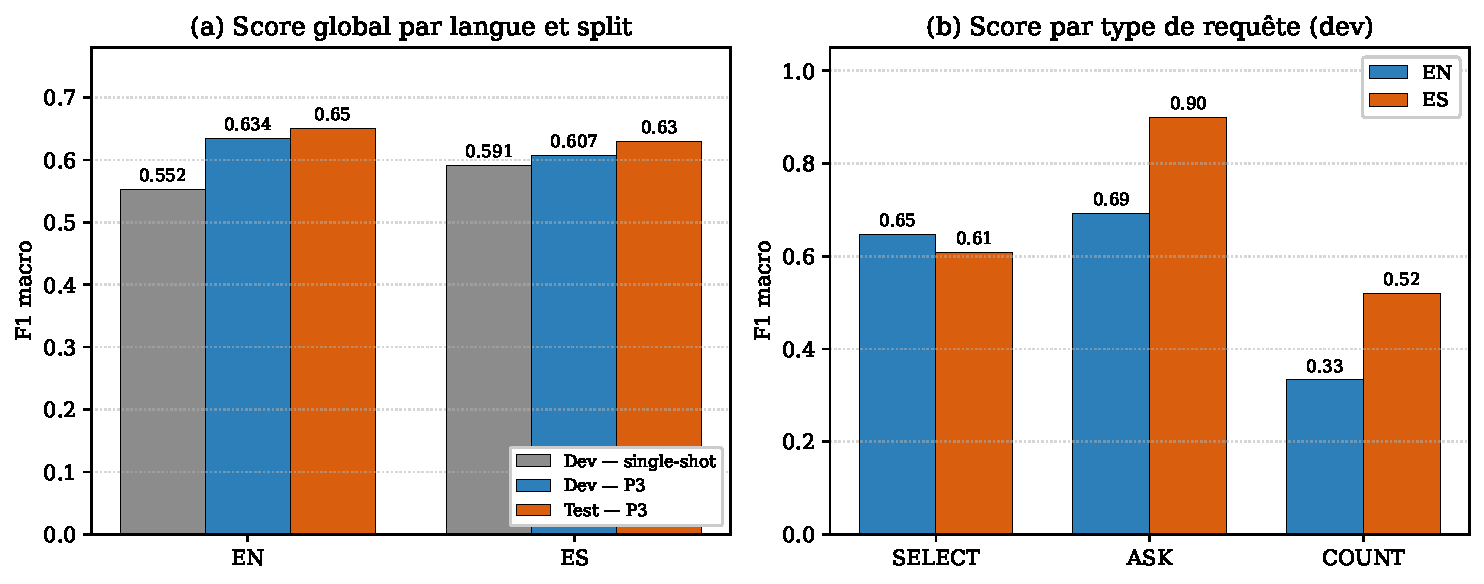
\includegraphics[width=0.95\linewidth]{results.pdf}
\caption{P3 results. (a)~Macro F1 by language and split: multi-candidate is more profitable in English than in Spanish, and test is in tight parity with dev. (b)~F1 by query type on the dev split: \texttt{ASK} is handled well (especially in Spanish), \texttt{COUNT} remains the weak spot.}
\label{fig:results}
\end{figure}

To quantify how brittle the retriever is under paraphrase, we also measure the Jaccard overlap between the top-3 neighbourhoods returned by TF-IDF and those of three modern sentence encoders (\texttt{all-MiniLM-L6-v2}, \texttt{bge-small-en-v1.5}, \texttt{bge-m3}~\cite{chen2024bge}). Average Jaccard hovers around 0.20 in all three cases, meaning that switching to a neural retriever would massively reconstruct the few-shot context; this is our main avenue for future improvement.

%==============================================================================
\section{Discussion}
\label{sec:discussion}
%==============================================================================
We cross P3's predictions with the generated query type and the dominant question word (Table~\ref{tab:bytypeinterr}). The two views do not overlap perfectly: the top block classifies questions by the SPARQL type that P3 actually produced, while the bottom block classifies them by their surface form (question word). This is why the \emph{how-many/cu\'antos} row does not exactly match the \texttt{COUNT} row — some \emph{``which''} questions really ask for a count (\emph{``which country has the most \ldots?''}) and result in a \texttt{COUNT} query. \texttt{COUNT} queries under-perform in both languages; the recurring failure mode is dropping the aggregate — the LLM emits \texttt{SELECT ?c WHERE \{~\dots~\}} instead of \texttt{SELECT (COUNT(?c) AS ?n) WHERE \{~\dots~\}}. Conversely, Spanish \texttt{ASK} questions reach 0.900: Spanish yes/no formulations (\emph{``\textnormal{\textquestiondown}Es \ldots?''}, \emph{``\textnormal{\textquestiondown}Tiene \ldots?''}) are more formally constrained than in English, which guides the model well. The sharpest observation is structurally identical in both languages: a single interrogative category accounts for half of the zeros. In English, \emph{``which''} questions represent 32\% of the dev split and 15 zeros out of 31; in Spanish, \emph{``qu\'e''} questions represent 39\% and 16 zeros out of 34. Both categories share the same logical structure: filter an entity set by its type, which passes through the \texttt{?x wdt:P31/wdt:P279* wd:Qtype} chain; this transitive closure is incomplete on the challenge endpoint. The LLM emits the plausible chain but execution returns zero rows. In contrast, short questions relying on a direct property (\emph{``when/cu\'ando''}, \emph{``who/qui\'en''}) are near-perfect because they rely on well-materialised properties such as \texttt{P569} (date of birth) or \texttt{P161} (cast). Two complementary gradients confirm this diagnosis: F1 drops by about 0.30 point between questions with two mentions and those with three or more, and by 0.16 point between short ($\leq 6$~words) and medium (7--10~words) questions, both effects converging with the \emph{``which/qu\'e''} category which is longer and more constrained on average. Finally, the profitability of multi-candidate breaks into three regimes: about 75\% of questions are solved on the first attempt; attempts 2--4 rescue effectively in English (mean F1 around 0.87) but marginally in Spanish (mean F1 around 0.30); when all five candidates return empty, no rescue happens and these 16--18 questions per language correspond to the homogeneous profile of \texttt{P31/P279*} chains. Three directions stand out for future work: a neural retriever (\texttt{bge-m3}) to capture paraphrases; a light profiling of the endpoint — one \texttt{SELECT ?p (COUNT(?o) AS ?n)} query per mentioned entity — to feed the LLM the list of actually available properties; a single-shot self-refinement pass~\cite{madaan2023selfrefine} on the specific questions where the five candidates all return empty.

\begin{table}[h]
\centering
\caption{Performance by SPARQL query type produced by P3 (top block) and dominant question word (bottom block) over the 100 dev questions in EN and ES. The top block sums to 100 per language; the bottom block omits an \emph{other} bucket (5 questions in EN, 9 in ES) that groups marginal question words.}
\label{tab:bytypeinterr}
\begin{tabular}{lcccccc}
\toprule
 & \multicolumn{3}{c}{EN} & \multicolumn{3}{c}{ES} \\
\cmidrule(lr){2-4}\cmidrule(lr){5-7}
Category & $n$ & F1 & Zero & $n$ & F1 & Zero \\
\midrule
\multicolumn{7}{l}{\emph{By SPARQL query type}} \\
SELECT   & 81 & 0.647 & 23 & 77 & 0.584 & 27 \\
ASK      & 13 & 0.692 &  4 & 10 & 0.900 &  1 \\
COUNT    &  6 & 0.333 &  4 & 13 & 0.520 &  6 \\
\midrule
\multicolumn{7}{l}{\emph{By dominant question word}} \\
which / qu\'e         & 32 & 0.425 & 15 & 39 & 0.470 & 16 \\
what / cu\'al         & 23 & 0.701 &  6 &  9 & 0.667 &  3 \\
who / qui\'en         & 13 & 0.822 &  1 & 13 & 0.800 &  2 \\
when / cu\'ando       &  9 & 1.000 &  0 &  9 & 0.889 &  1 \\
how-many / cu\'antos  &  5 & 0.200 &  4 & 10 & 0.400 &  6 \\
yes-no                & 13 & 0.692 &  4 & 10 & 0.900 &  1 \\
\bottomrule
\end{tabular}
\end{table}

%==============================================================================
\section{Conclusion}
\label{sec:conclusion}
%==============================================================================
We have presented a deliberately simple pipeline for question-to-SPARQL conversion on Wikidata, applied to the two \emph{with-mentions} tracks of the WikiKGQA~@~ISWC~2026 challenge. By chaining TF-IDF retrieval, a three-example few-shot prompt, generation of five candidates at mixed temperatures, and execution-guided selection on the challenge endpoint, the system reaches macro F1 of 0.634 in English and 0.607 in Spanish on the dev split, and respectively 0.650 and 0.630 on the official Codabench test, while using only freely available open-weight LLMs. The error analysis identifies two resistant categories — type-filter questions in \emph{``which/qu\'e''}, defeated by the \texttt{P31/P279*} transitive closure being incomplete on the endpoint, and \texttt{COUNT} queries for which the LLM drops the aggregate — and opens three targeted directions: a neural retriever to capture paraphrases, a light endpoint profile to avoid non-materialised properties, and a conditional self-refinement round for the questions where multi-candidate has failed to recover the answer. The code, data and Codabench archives are released at \url{https://github.com/emeric-cyrille/wikikgqa-iswc2026}.

%==============================================================================
\bibliography{main}
%==============================================================================

\end{document}
